\documentclass[12pt]{article}
% Change ``article'' to ``report'' to get rid of page number on title page
\usepackage{amsmath,amsfonts,amsthm,amssymb}
\usepackage{fancyhdr}
\usepackage{lastpage}
\usepackage{extramarks}
\usepackage{soul,color}
\usepackage{titlesec}
\usepackage{graphicx,float,wrapfig}
\usepackage{url}

% In case you need to adjust margins:
\topmargin=-0.45in      %
\evensidemargin=-1in     %
\oddsidemargin=0in      %
\textwidth=7in        %
\textheight=9.0in       %
\headsep=0.25in         %

% Start of document. 
\begin{document}
\begin{center}                  % Header of file. 
\textbf{\Large{Lexis Issue Library Project}} \\ 
\small\textsc{Shumin Guo} \\
\today
\end{center}

%% Overview. 
\section{Project Overview.}
Legal citations are important in issue documents, previous work on
issue citation network has been proved to be effective to utilize the
citing relationship. One reason for the limited use of legal issue
citation is that the citation link of two legal issue documents is
asymmetric. For example, at one end of the citation link is the reason
for citation (RFC), while on the other end, it is the whole case
Case_X:CiteArea_A --> Case_Y. It is not clear which area Case_X is
citing in Case_Y.

In this project, we try to implement a framework called "Semantics
Based Citation Pairing." We introduced a new type of legal metadata,
legal issues based on case-law documents, we believe that such a
metadata database could support efforts parallel to current trends of
technology, and the citation pairing metadata would also enable other
potential functions and data creation that assist legal analytics, and
thus this would benefit legal researchers by deepening analytics from
the document level into a more semantic level of legal issues. And our
previous work at NTR has shown that, through some kind of processing,
much of the missing information can be filled into the picture. And as
a result the citation between two cases become from Case_X:CiteArea_A
--> Case_Y to Case_X:CiteArea_A --> Case_Y:CiteArea_B.  

%% daily routines. 
\section{Project Workflow.}
Generally, this project can be splitted into the following steps. 
\begin{itemize}
\item Data extraction from xml files, citation meta-data and paragraph
  data will be extracted during this step. 
\item Sentence cutting, which cuts the paragraphic text into
  sentences. 
\item RFC Segmentation, which extracts segmented Reason For Citation
  data from sentences around the citation point. 
\item RFC vector normalization, which normalizes the RFC vector. 
\item Vector comparison, which compares the similarities of the
  vectors and output a quantitive similarity value. 
\item Building LIL from vector comparison table. 
\end{itemize}

For detailed processing steps and data flow, please see Figure
\ref{fig:proj_flow}. 

\begin{figure}[t]
\centering
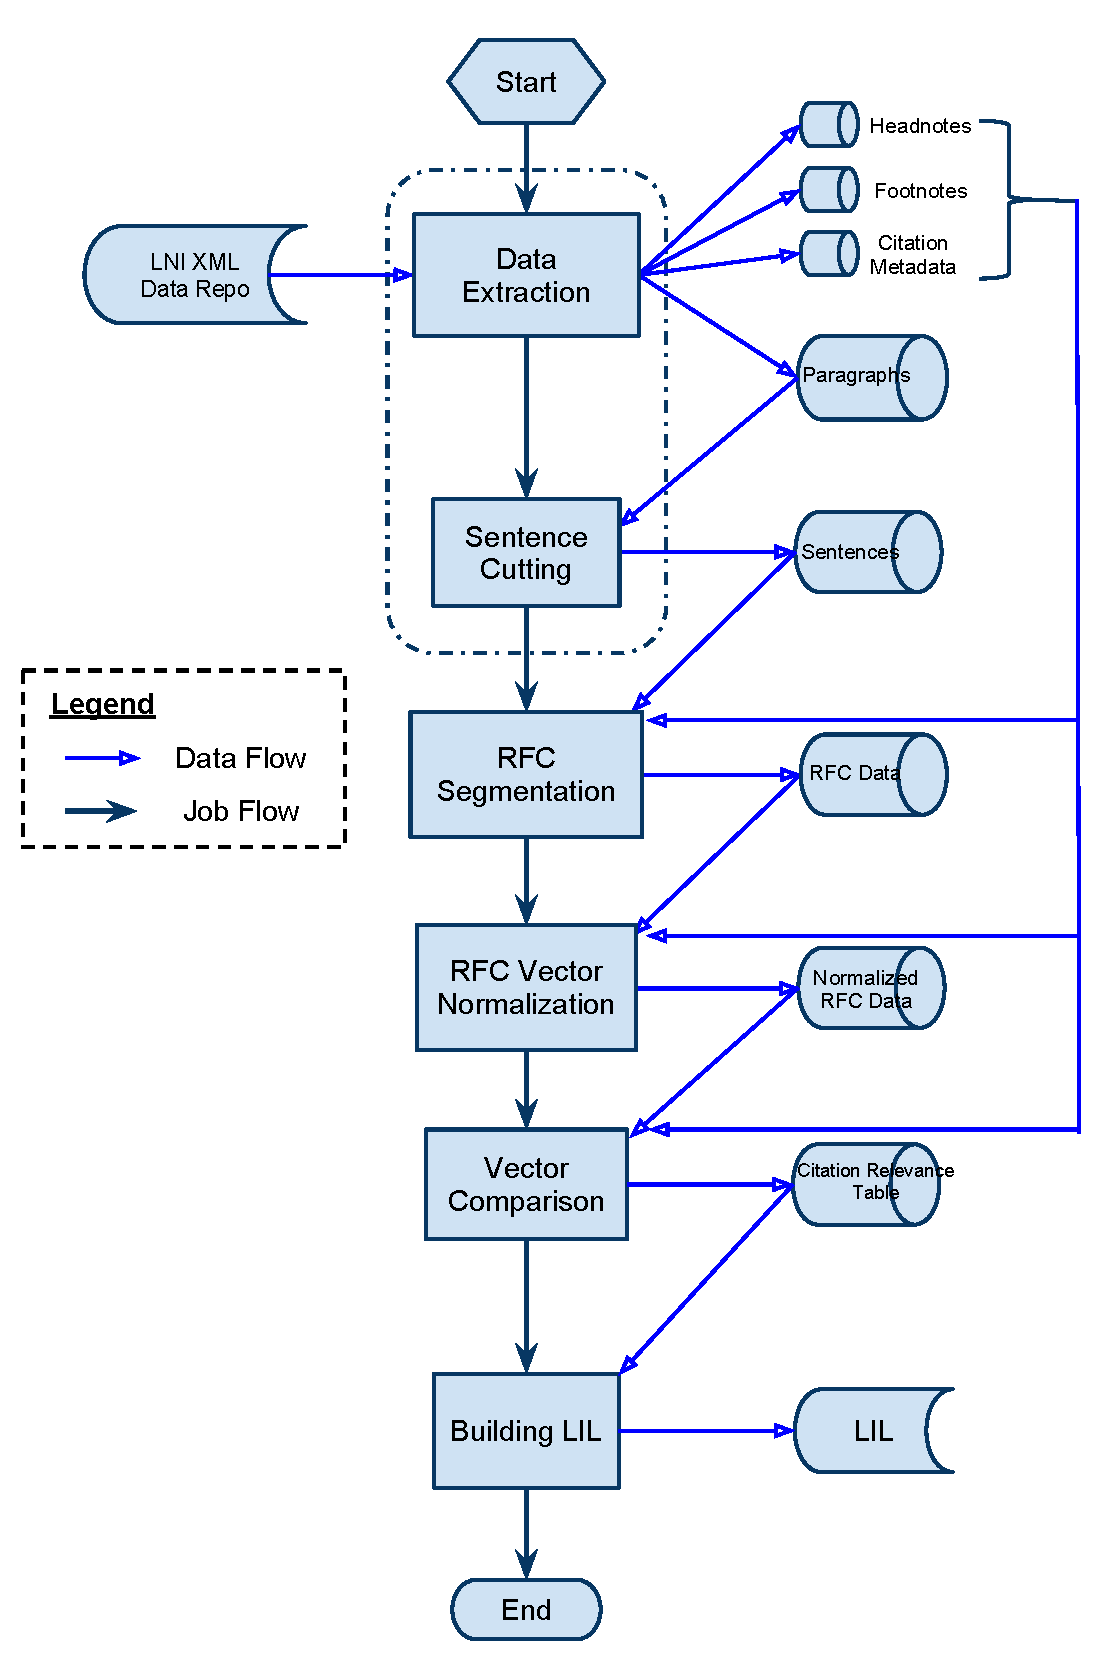
\includegraphics[width=1.0\textwidth]{LILFlowChart.pdf}
\caption{Flow Chart of LIL Project.}
\label{fig:proj_flow}
\end{figure}

%% The working environment. 
\section{Project Implementation Design.}

%% valiation. 
\section{Project and Step-wise Verification}

\section{Project Technics and Software}


\end{document}
